% Options for packages loaded elsewhere
\PassOptionsToPackage{unicode}{hyperref}
\PassOptionsToPackage{hyphens}{url}
%
\documentclass[
  ignorenonframetext,
]{beamer}
\usepackage{pgfpages}
\setbeamertemplate{caption}[numbered]
\setbeamertemplate{caption label separator}{: }
\setbeamercolor{caption name}{fg=normal text.fg}
\beamertemplatenavigationsymbolsempty
% Prevent slide breaks in the middle of a paragraph
\widowpenalties 1 10000
\raggedbottom
\setbeamertemplate{part page}{
  \centering
  \begin{beamercolorbox}[sep=16pt,center]{part title}
    \usebeamerfont{part title}\insertpart\par
  \end{beamercolorbox}
}
\setbeamertemplate{section page}{
  \centering
  \begin{beamercolorbox}[sep=12pt,center]{part title}
    \usebeamerfont{section title}\insertsection\par
  \end{beamercolorbox}
}
\setbeamertemplate{subsection page}{
  \centering
  \begin{beamercolorbox}[sep=8pt,center]{part title}
    \usebeamerfont{subsection title}\insertsubsection\par
  \end{beamercolorbox}
}
\AtBeginPart{
  \frame{\partpage}
}
\AtBeginSection{
  \ifbibliography
  \else
    \frame{\sectionpage}
  \fi
}
\AtBeginSubsection{
  \frame{\subsectionpage}
}
\usepackage{amsmath,amssymb}
\usepackage{lmodern}
\usepackage{iftex}
\ifPDFTeX
  \usepackage[T1]{fontenc}
  \usepackage[utf8]{inputenc}
  \usepackage{textcomp} % provide euro and other symbols
\else % if luatex or xetex
  \usepackage{unicode-math}
  \defaultfontfeatures{Scale=MatchLowercase}
  \defaultfontfeatures[\rmfamily]{Ligatures=TeX,Scale=1}
\fi
% Use upquote if available, for straight quotes in verbatim environments
\IfFileExists{upquote.sty}{\usepackage{upquote}}{}
\IfFileExists{microtype.sty}{% use microtype if available
  \usepackage[]{microtype}
  \UseMicrotypeSet[protrusion]{basicmath} % disable protrusion for tt fonts
}{}
\makeatletter
\@ifundefined{KOMAClassName}{% if non-KOMA class
  \IfFileExists{parskip.sty}{%
    \usepackage{parskip}
  }{% else
    \setlength{\parindent}{0pt}
    \setlength{\parskip}{6pt plus 2pt minus 1pt}}
}{% if KOMA class
  \KOMAoptions{parskip=half}}
\makeatother
\usepackage{xcolor}
\newif\ifbibliography
\usepackage{graphicx}
\makeatletter
\def\maxwidth{\ifdim\Gin@nat@width>\linewidth\linewidth\else\Gin@nat@width\fi}
\def\maxheight{\ifdim\Gin@nat@height>\textheight\textheight\else\Gin@nat@height\fi}
\makeatother
% Scale images if necessary, so that they will not overflow the page
% margins by default, and it is still possible to overwrite the defaults
% using explicit options in \includegraphics[width, height, ...]{}
\setkeys{Gin}{width=\maxwidth,height=\maxheight,keepaspectratio}
% Set default figure placement to htbp
\makeatletter
\def\fps@figure{htbp}
\makeatother
\setlength{\emergencystretch}{3em} % prevent overfull lines
\providecommand{\tightlist}{%
  \setlength{\itemsep}{0pt}\setlength{\parskip}{0pt}}
\setcounter{secnumdepth}{-\maxdimen} % remove section numbering
\ifLuaTeX
  \usepackage{selnolig}  % disable illegal ligatures
\fi
\IfFileExists{bookmark.sty}{\usepackage{bookmark}}{\usepackage{hyperref}}
\IfFileExists{xurl.sty}{\usepackage{xurl}}{} % add URL line breaks if available
\urlstyle{same} % disable monospaced font for URLs
\hypersetup{
  pdftitle={Redistricting},
  pdfauthor={Brian Holland, Brad Wayne, Kumar Himanshu, Grace Edna, Chuyuan Zhong},
  hidelinks,
  pdfcreator={LaTeX via pandoc}}

\title{Redistricting}
\author{Brian Holland, Brad Wayne, Kumar Himanshu, Grace Edna, Chuyuan
Zhong}
\date{12/4/2022}

\begin{document}
\frame{\titlepage}

\begin{frame}{Problem}
\protect\hypertarget{problem}{}
\begin{itemize}
\tightlist
\item
  Investigating the affects of states' redistricting stance on voter
  turnout.
\end{itemize}

\begin{figure}
\centering
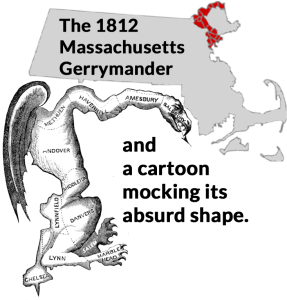
\includegraphics{images/GerryManderCartoonMap.png}
\caption{Original Gerrymander}
\end{figure}
\end{frame}

\begin{frame}{}
\protect\hypertarget{section}{}
\begin{figure}
\centering
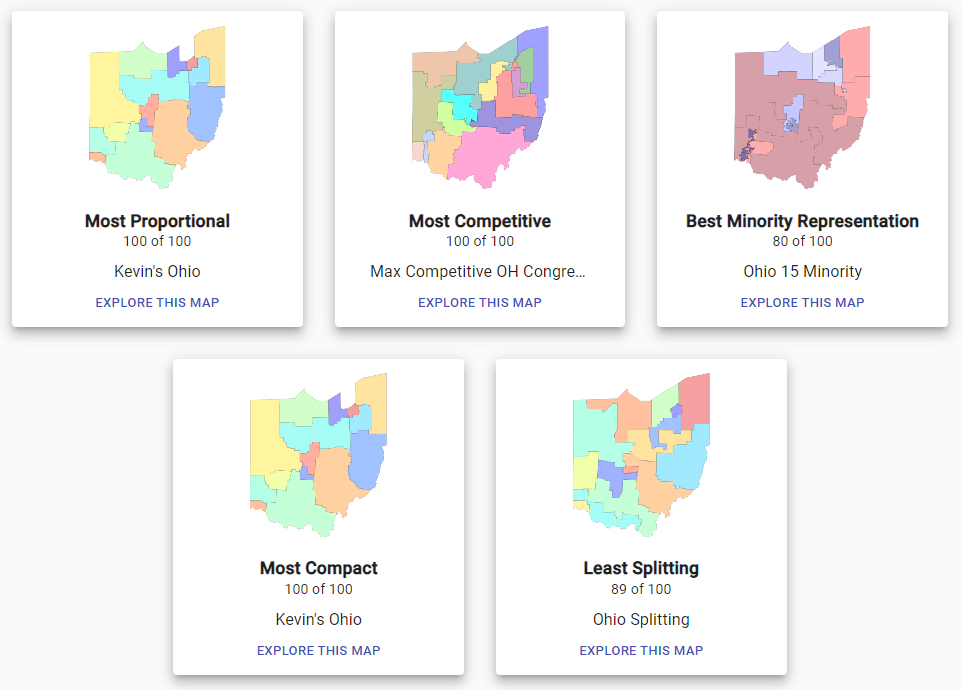
\includegraphics{images/ohio_bests.png}
\caption{Best Ohio maps}
\end{figure}
\end{frame}

\begin{frame}{}
\protect\hypertarget{section-1}{}
\begin{figure}
\centering
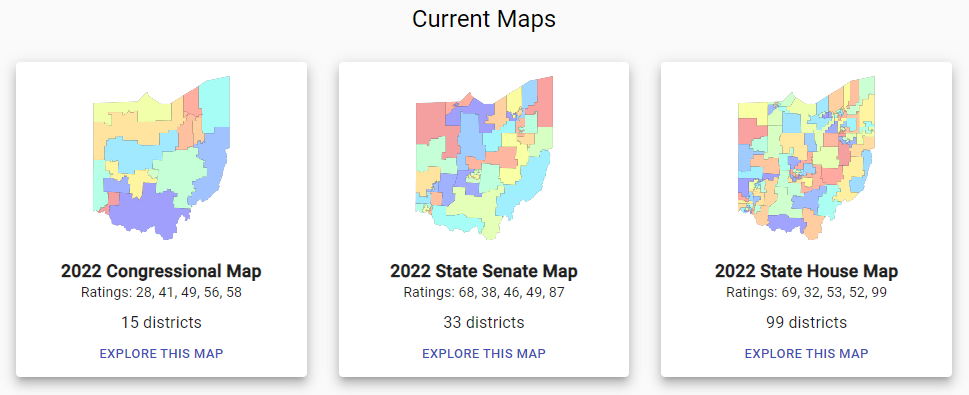
\includegraphics{images/ohio_current.png}
\caption{Ohio's illegal maps}
\end{figure}
\end{frame}

\begin{frame}{Problem}
\protect\hypertarget{problem-1}{}
\begin{itemize}
\item
  ``Redistricting'' in the US - normal, decennial process through states
  redraw the boundaries of districts
\item
  Concerns about fairness (In a perfect world, the lines would be drawn
  in the fairest way possible. But even that is hard to measure and
  execute, depending on your version of ``fair'')
\item
  How the lines are drawn might influence election outcomes.(There is
  very little guidance and even fewer rules about what the line-drawing
  process is supposed to be, and the lines can easily be drawn to favor
  your party over the other.)
\item
  Recent increase in partisan polarization, role of redistricting (The
  ``guardrail'' of democratic behavior usually meant moderate gains
  losses during redistricting, knowing your party might not be in power
  in 10 years. But recently, tactics have grown fiercely partisan in
  many cases).
\end{itemize}
\end{frame}

\begin{frame}{}
\protect\hypertarget{section-2}{}
\begin{figure}
\centering
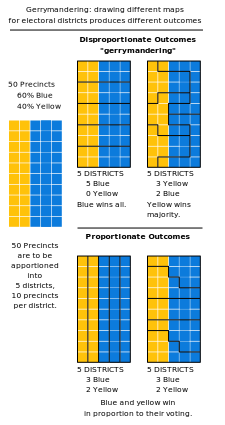
\includegraphics[width=0.35\textwidth,height=\textheight]{images/DifferingApportionment.svg}
\caption{Redistricting illustrated}
\end{figure}
\end{frame}

\begin{frame}{Terminology}
\protect\hypertarget{terminology}{}
\begin{itemize}
\tightlist
\item
  Legislature
\item
  Commission
\item
  Courts
\item
  Exceptions (single-district states, etc)
\end{itemize}

\#\#Background

\#\#Theory

\begin{itemize}
\tightlist
\item
  Non-partisan redistricting methods should lead to higher turnout.
\end{itemize}
\end{frame}

\begin{frame}{Data Sources}
\protect\hypertarget{data-sources}{}
\begin{block}{1. Congressional election data, 2000-2020}
\protect\hypertarget{congressional-election-data-2000-2020}{}
\begin{itemize}
\tightlist
\item
  MIT Election Lab
\item
  Level: Congressional District
\end{itemize}
\end{block}
\end{frame}

\begin{frame}{\#\#\# 2. Redistricting policies by state, 2000-2020}
\protect\hypertarget{redistricting-policies-by-state-2000-2020}{}
\begin{block}{3. US Census turnout}
\protect\hypertarget{us-census-turnout}{}
\end{block}
\end{frame}

\begin{frame}{Data cleaning and merging}
\protect\hypertarget{data-cleaning-and-merging}{}
\begin{itemize}
\item
  Drop with states with only one district
\item
  {[}Redistricting cleaning{]}
\item
\end{itemize}
\end{frame}

\end{document}
